\documentclass[a4paper]{article}
\usepackage[french]{babel}
\usepackage[utf8]{inputenc}
\usepackage[T1]{fontenc}
\usepackage{todonotes}
\usepackage{graphicx}
\usepackage{subcaption}
\usepackage{amssymb} % nécessaire pour \mathbb
\usepackage{mathtools}
\usepackage{csquotes}
\usepackage{hyperref}
\usepackage[style=ieee]{biblatex}
\addbibresource{ref.bib}
\bibliography{ref.bib}

\renewcommand\UrlFont{\color{blue}\rmfamily}

\title{Etat de l'art des réseaux de convolutions de graphes et leurs nuances.}
\author{Cléa HAN - Léa TRIQUET - Adrien ZABBAN}
\date{27 octobre 2023}

\begin{document}
\maketitle

\section{Introduction}

Les méthodes que l'ont va aborder:
\begin{itemize}
    \item Graph Convolusional Networks~\cite{DBLP:journals/corr/KipfW16} (GCN)
    \item Simplifying Graph Convolutional Networks~\cite{DBLP:journals/corr/abs-1902-07153} (SGC)
    \item Graph Isomorphism Network~\cite{DBLP:journals/corr/abs-1810-00826} (GIN)
\end{itemize}

\section{Les différentes méthodes}

\subsection{Graph Convolusional Networks (GCN)}\label{sec: GCN}
Un Graph Convolution Network (GCN) est un type de réseau de neurones artificiels conçu pour traiter des données 
structurées sous forme de graphes. Ils utilisent des opérations de convolution spécialement adaptées aux graphes 
pour propager l'information entre les nœuds du graphe, ce qui leur permet de capturer les relations et les 
dépendances entre les entités interconnectées. L'équation~\ref{eq: propragation de couche} représente la règle de
propagation de la couche $l$ à la couche $l+1$.
\begin{equation}
    H^{(l-1)} = \sigma (\Tilde{D}^{-\frac{1}{2}} \Tilde{A} \Tilde{D}^{-\frac{1}{2}} H^{(l)} W^{(l)})
    \label{eq: propragation de couche}
\end{equation}
où $\Tilde{A}=A+I_n$ est la matrice d'adjacence au quelle on ajoute des connections sur les noeuds vers 
eux-mêmes. $\Tilde{D_{ii}}=\sum_j{\Tilde{A_{ij}}}$ qui est une matrice diagonale des degrés des noeuds du 
graphe. $W^{(l)}$ sont les poids de la couche $l$ et $H^{(l)}$ est la sortie de la couche $l-1$, $H^{(0)}=X$. 
$\sigma$ est une fonction d'activation.

Par exemple, un petit réseaux de convolutions de graphes pourait suivre l'équation~\ref{eq: reseaux de 2 GCN}
\begin{equation}
    Z_{GCN} = \text{softmax}(\hat{A}\,\text{ReLU}(\hat{A}XW^{(0)})W^{(1)})
    \label{eq: reseaux de 2 GCN}
\end{equation}
où $\hat{A} = \Tilde{D}^{-\frac{1}{2}} \Tilde{A} \Tilde{D}^{-\frac{1}{2}}$



\subsection{Simplifying Graph Convolutional Networks (SGC)}

Les modèles SGCs sont construits à partir d'une linéarisation des GCNs en faisant l'hypothèse que les non linéarités 
principalement apportées par les ReLU entre les différentes couches d'un GCN n'apportent pas d'informations significatives.
 Ainsi, les modèles SGCs retirent ces non linéarités et conservent uniquement un Softmax en dernière couche, afin de pouvoir 
 obtenir des résultats sous forme d'une distribution de probabilités.

Nous pouvons modéliser le SGC sous la forme de l'expression simplifiée suivante l'équiation~\ref{eq: SGC}
\begin{equation}
  Z_{SGC}=\text{softmax}(\hat{A}^KXW)
  \label{eq: SGC}
\end{equation}
où $\hat{A}^K$ représentant les $K$ multiplications successives avec $\hat{A}$ notre matrice d'adjacence normalisée,
définie dans la section~\ref{sec: GCN}, $X$ est les entrées 
et $W$ est la matrice réunissant l'ensemble des poids utilisés dans le modèle tel que : $W=W^{(1)} W^{(2)} \dots W^{(K)}$.
La SGC équivaut à une une composante d'extraction de caractéristiques: $\tilde{X}=\hat{A}^KX$, ce qui nécessite aucun 
poids. Puis, cela est suivi d'une régression logistique $Z_{SGC}=\text{softmax}(\tilde{X}W)$. Ainsi la première étape équivaut 
à du prétraitement des caractéristiques de nos données $X$, car aucun poids n'est appliqué sur nos données. Ainsi, l'entraînement
 du SGC s'apparente en réalité à une régression logistique multi classe sur des données prétraités. 
D'autre part, l'entraînement d'une régression logistique est un problème d'optimisation convexe bien documenté, ainsi ses 
performances seront relativement meilleures que celles du GCN qui contient des non linéarités. De plus, l'entraînement du 
SGC sera naturellement plus rapide.
D'un point de vue “graphe”, la SGC correspond à un filtre fixe sur le domaine du graphe spectral. Si nous ajoutons des boucles 
dans le graphe original, l'application du SGC permet de réduire la taille du spectre graphique grâce à l'astuce de renormalisation 
présentée par Kipf \& Welling~\cite{DBLP:journals/corr/KipfW16}. La SGC agit comme un filtre passe bas qui lasse les 
caractéristiques du graphes, ainsi les 
nœuds voisins vont avoir tendance à partager des représentations et donc des prédictions similaires. 


\subsection{Graph Isomorphism Network (GIN)}

\section{Entraînements}

Nous avons entraîné des petits réseaux de neurones utilisant les GCN, SGC et GIN. La
Figure~\ref{fig:entrainement} représente respectivement l'entrainement des modèles 
GCN, SGC et GIN.


\begin{figure}[ht]
    \centering
    \begin{subfigure}{0.47\textwidth}
      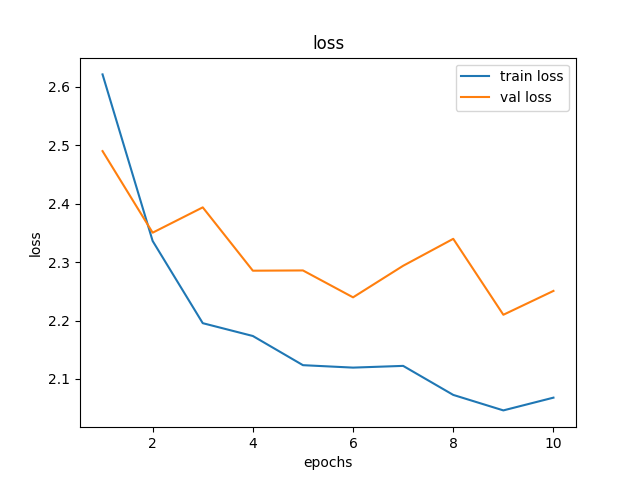
\includegraphics[width=\linewidth]{../results/GCN_0/loss.png}
      \caption{GCN: Cross Entropy Loss}
    \end{subfigure}
    \hfill
    \begin{subfigure}{0.47\textwidth}
      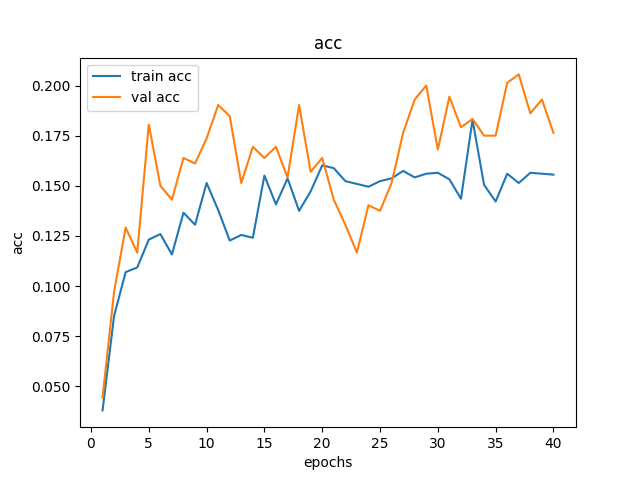
\includegraphics[width=\linewidth]{../results/GCN_0/acc.png}
      \caption{GCN: accuracy}
    \end{subfigure}\\

    \begin{subfigure}{0.47\textwidth}
      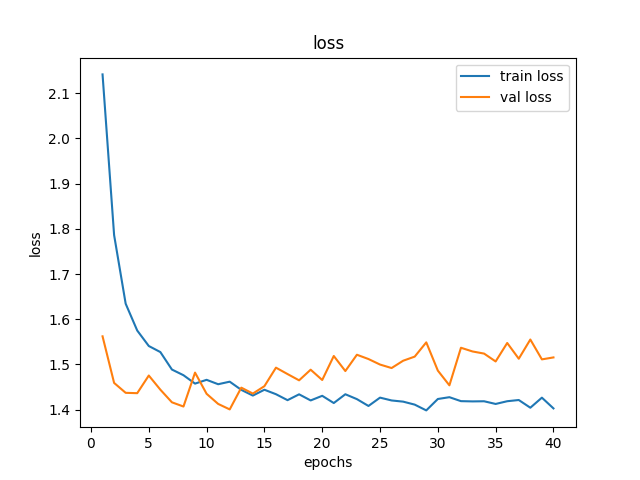
\includegraphics[width=\linewidth]{../results/SGC_1/loss.png}
      \caption{SGC: Cross Entropy Loss}
    \end{subfigure}
    \hfill
    \begin{subfigure}{0.47\textwidth}
      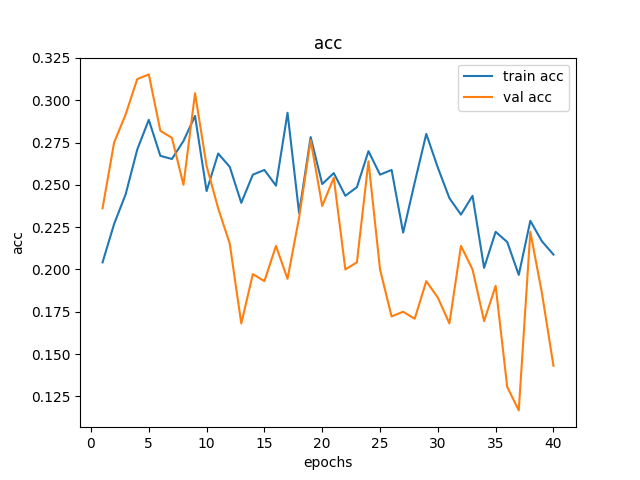
\includegraphics[width=\linewidth]{../results/SGC_1/acc.png}
      \caption{SGC: accuracy}
    \end{subfigure}\\

    \begin{subfigure}{0.47\textwidth}
      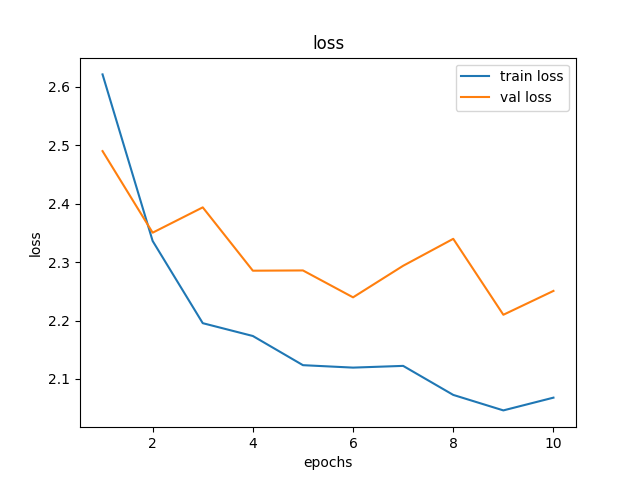
\includegraphics[width=\linewidth]{../results/GCN_0/loss.png}
      \caption{GIN: Cross Entropy Loss}
    \end{subfigure}
    \hfill
    \begin{subfigure}{0.47\textwidth}
      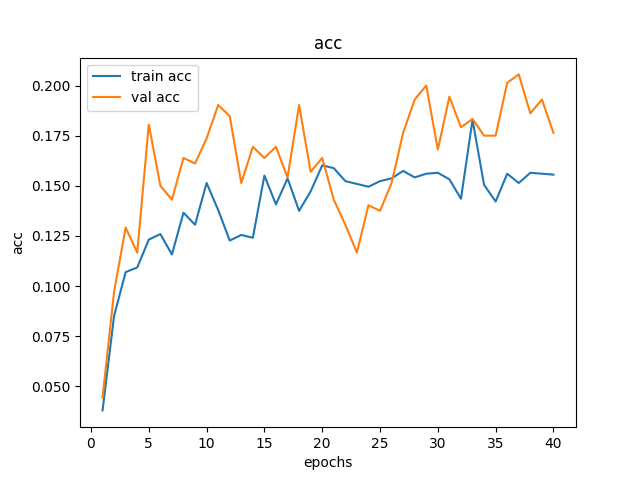
\includegraphics[width=\linewidth]{../results/GCN_0/acc.png}
      \caption{GIN: accuracy}
    \end{subfigure}
    \caption{Entraînement des modèles GCN, SGC et GIN}
    \label{fig:entrainement}
  \end{figure}


\section{Résultats et conclusion}

Nous voyons sur la Table~\ref{tab:test}, les résultats des modèles sur la base de données de teste.

\begin{table}
    \centering
    \begin{tabular}{|c|c|c|c|}
        \hline
        Modèles & GCN & SGC & GIN \\
        \hline
        Cross Entropy & 2.86 & 1.85 & 1.75 \\
        \hline
        Accuracy & 0.20 & 0.16 & 0.38\\
        \hline
    \end{tabular}
    \caption{Résultat sur la base de données de teste}
    \label{tab:test}
\end{table}

\newpage
\printbibliography

\end{document}
